\documentclass[UTF8,a4paper,12pt]{ctexart}

\usepackage[left=2.3cm,right=2.3cm,top=2.6cm,bottom=2.6cm]{geometry}
\usepackage{amsmath,amssymb,bm}
\usepackage{booktabs}
\usepackage{array}
\usepackage{multirow}
\usepackage{float}
\usepackage{graphicx}
\usepackage{xcolor}
\usepackage{hyperref}
\usepackage{caption}
\usepackage{longtable}
\usepackage{siunitx}
\usepackage{enumitem}
\usepackage{pgfplots}
\usepackage{tikz}
\usetikzlibrary{positioning,shapes,arrows.meta,calc}
\pgfplotsset{compat=1.18}

\hypersetup{
  colorlinks=true,
  linkcolor=blue,
  citecolor=blue,
  urlcolor=blue
}

\title{\textbf{基于DDPG的双足机器人行走控制实验报告}}
\author{姓名：\underline{邓一骏\hspace{3cm}} \quad 学号：\underline{25SD36037\hspace{3cm}}}
\date{\today}

\begin{document}

\maketitle
\tableofcontents
\newpage

\section{实验目标}

本实验以OpenAI Gymnasium中的双足机器人行走任务\texttt{BipedalWalker-v3}为研究对象，采用深度确定性策略梯度算法（Deep Deterministic Policy Gradient, DDPG），实现智能体对连续动作空间下机器人行走策略的学习。

\paragraph{核心研究问题：}
如何在连续动作空间中，通过Actor-Critic结构、经验回放与目标网络机制，使双足机器人学会稳定、高效的行走策略，并在合理训练预算内达到环境求解标准（评估平均回报$\geq 300$）。

\paragraph{量化评价指标：}
\begin{itemize}[leftmargin=2em]
  \item \textbf{训练累计回报}（Train Reward）：每个episode内所有即时奖励之和。
  \item \textbf{平滑回报}（Smoothed Reward）：取窗口$K=10$的滑动平均，用于消除噪声反映趋势。
  \item \textbf{评估平均回报}（Eval Reward）：每20个训练回合，在无探索噪声条件下运行5个episode的平均回报。
  \item \textbf{求解标准}：评估平均回报$\geq 300$视为环境解决。
\end{itemize}

\section{环境与问题描述}

\subsection{任务背景}

\texttt{BipedalWalker-v3}是Gymnasium框架中标准的连续控制测试环境，要求智能体控制一个双足机器人在起伏地形上前进。该环境具有如下技术特征：
\begin{itemize}[leftmargin=2em]
  \item \textbf{观测空间}（Observation Space）：24维连续向量，包含机体姿态角、角速度、关节角度与角速度、足底接触状态及前方地形LIDAR测距信息。
  \item \textbf{动作空间}（Action Space）：4维连续向量，每个维度取值$[-1, 1]$，对应四个关节电机的归一化扭矩输出。
  \item \textbf{奖励函数}：由前进速度奖励、能耗惩罚和姿态稳定性惩罚三部分构成。每前进一步获得正向奖励，电机过度使用产生负向惩罚，机体倾斜过大或跌倒时给予强负奖励并终止回合。
  \item \textbf{终止条件}：机器人躯干触地、头部高度过低、达到最大步数（1600步）、或成功到达终点。
\end{itemize}

\subsection{核心难点}

\begin{enumerate}[leftmargin=2em]
  \item \textbf{连续动作空间：}无法通过离散动作枚举进行Q-Learning，必须使用确定性策略梯度方法或随机策略方法。
  \item \textbf{高维连续状态：}24维观测空间需要神经网络具备有效的特征提取能力。
  \item \textbf{探索与利用的平衡：}随机探索过强容易导致频繁摔倒，探索过弱则无法发现有效行走策略。
  \item \textbf{训练稳定性：}Actor与Critic同时更新易导致值函数高估、梯度震荡和目标不匹配问题。
  \item \textbf{奖励稀疏性与延迟性：}初期大量负奖励掩盖了策略改进的信号，需要较长的训练周期才能观察到正向回报。
\end{enumerate}

\section{算法原理}

\subsection{DDPG算法概述}

DDPG\cite{lillicrap2015ddpg}是一种面向连续动作空间的off-policy Actor-Critic算法。它将深度Q网络（DQN）的经验回放与目标网络思想扩展到连续控制领域，结合确定性策略梯度（Deterministic Policy Gradient, DPG）\cite{silver2014dpg}实现对连续动作的直接优化。

将双足机器人控制问题建模为马尔可夫决策过程（MDP）：
\[
\mathcal{M} = (\mathcal{S}, \mathcal{A}, P, R, \gamma)
\]
其中状态空间$\mathcal{S} \subset \mathbb{R}^{24}$，动作空间$\mathcal{A} \subset \mathbb{R}^{4}$，$\gamma = 0.99$为折扣因子。目标是学习确定性策略$\mu_\theta: \mathcal{S} \to \mathcal{A}$最大化期望累计折扣回报：
\[
J(\theta) = \mathbb{E}_{s_0 \sim \rho_0}\left[\sum_{t=0}^{\infty} \gamma^t r(s_t, \mu_\theta(s_t))\right]
\]

\subsection{Actor-Critic架构}

\paragraph{Actor网络（策略网络）}
Actor $\mu(s|\theta^\mu)$将状态映射到确定性动作，采用双隐层全连接结构：
\begin{equation}
a_t = \tanh(h_2(W_2 \cdot \text{ReLU}(W_1 s + b_1) + b_2)) \cdot a_{\max}
\end{equation}
其中$W_1 \in \mathbb{R}^{400 \times 24}$, $W_2 \in \mathbb{R}^{300 \times 400}$，输出层使用$\tanh$将动作约束在$[-1,1]$后乘以动作上界$a_{\max}$。

\paragraph{Critic网络（价值网络）}
Critic $Q(s,a|\theta^Q)$评估状态-动作对的价值，将状态与动作拼接后输入：
\begin{equation}
Q(s,a) = W_4 \cdot \text{ReLU}(W_3 \cdot [s, a] + b_3) + b_4
\end{equation}
其中$W_3 \in \mathbb{R}^{400 \times 28}$, $W_4 \in \mathbb{R}^{1 \times 300}$，输出为标量Q值。

\subsection{训练机制}

\paragraph{经验回放}
采用经验回放池$\mathcal{D}$存储转移样本$(s_t, a_t, r_t, s_{t+1}, d_t)$。训练时随机采样$N$个样本，打破时间相关性并提高样本利用率。

\paragraph{目标网络与软更新}
为Actor和Critic分别维护目标网络$\mu'$和$Q'$，参数通过Polyak平均软更新：
\begin{equation}
\theta^{Q'} \leftarrow \tau \theta^Q + (1-\tau)\theta^{Q'}, \quad
\theta^{\mu'} \leftarrow \tau \theta^\mu + (1-\tau)\theta^{\mu'}
\end{equation}
其中$\tau = 0.005$为软更新系数，取值较小以保证目标值缓慢变化。

\paragraph{Loss函数}

Critic通过最小化Bellman误差更新：
\begin{equation}
L_Q = \frac{1}{N}\sum_{i=1}^{N}\left(y_i - Q(s_i, a_i)\right)^2
\end{equation}
其中目标值$y_i = r_i + \gamma (1-d_i) Q'(s_{i+1}, \mu'(s_{i+1}))$。

Actor通过最大化Critic对当前策略动作的评价更新：
\begin{equation}
\nabla_{\theta^\mu} J \approx \frac{1}{N}\sum_{i=1}^{N}
\nabla_a Q(s,a)\big|_{s_i, \mu(s_i)}
\nabla_{\theta^\mu} \mu(s)\big|_{s_i}
\end{equation}

\subsection{探索噪声与稳定性增强}

\paragraph{Ornstein-Uhlenbeck噪声}
采用时间相关的OU过程作为探索噪声，相比高斯噪声能够在连续动作中维持动作趋势，更适合物理控制任务：
\begin{equation}
\mathrm{d}x_t = \theta(\mu - x_t)\mathrm{d}t + \sigma \mathrm{d}W_t
\end{equation}
其中$\theta=0.15$控制均值回归速度，$\sigma=0.20$控制噪声幅度。

\paragraph{目标策略平滑}
在计算目标Q值时，对目标动作添加裁剪后的高斯噪声：
\begin{equation}
\tilde{a}' = \text{clip}(\mu'(s') + \epsilon, -a_{\max}, a_{\max}), \quad
\epsilon \sim \text{clip}(\mathcal{N}(0, \sigma_p^2), -c, c)
\end{equation}
其中$\sigma_p = 0.20$为策略噪声标准差，$c = 0.50$为噪声裁剪范围。该技术通过平滑Q函数曲面有效减少值函数高估偏差\cite{fujimoto2018td3}。

\paragraph{梯度裁剪}
对Actor和Critic的梯度均进行裁剪：$\|\nabla_{\theta}L\|_2 \leq 1.0$，防止梯度爆炸导致的训练发散。

\begin{figure}[H]
\centering
\begin{tikzpicture}[node distance=0.8cm, auto]
\tikzset{
    block/.style={rectangle, rounded corners, draw=blue!60, thick, align=center, minimum width=2.8cm, minimum height=0.8cm, fill=blue!5},
    decision/.style={diamond, draw=orange!70, thick, aspect=1.8, align=center, fill=orange!10},
    process/.style={rectangle, draw=green!50!black, thick, rounded corners, align=center, minimum width=2.8cm, minimum height=0.8cm, fill=green!5},
    arrow/.style={->, thick, >=Stealth}
}
\node[block] (state) {环境状态 $s_t$};
\node[block, below=of state] (actor) {Actor $\mu(s_t)$};
\node[block, right=0.8cm of actor] (noise) {+ OU噪声};
\node[process, below=of noise] (action) {动作 $a_t$};
\node[block, below=of action] (env) {环境交互};
\node[block, right=0.8cm of env] (store) {存储 $\mathcal{D}$};
\node[decision, below=0.6cm of env] (update) {满足更新条件？};
\node[process, below left=0.6cm and 0.5cm of update] (sample) {采样 $N$ 条};
\node[block, below=of sample] (critic) {更新 Critic};
\node[block, below=of critic] (actor_up) {更新 Actor};
\node[block, below=of actor_up] (soft) {软更新目标网络};
\node[process, below right=0.6cm and 1.0cm of update] (continue) {继续探索};

\draw[arrow] (state) -- (actor);
\draw[arrow] (actor) -- (noise);
\draw[arrow] (noise) -- (action);
\draw[arrow] (action) -- (env);
\draw[arrow] (env) -- node[above]{$(s,a,r,s',d)$} (store);
\draw[arrow] (store) |- (update);
\draw[arrow] (update) -- node[left]{是} (sample);
\draw[arrow] (sample) -- (critic);
\draw[arrow] (critic) -- (actor_up);
\draw[arrow] (actor_up) -- (soft);
\draw[arrow] (soft.west) -- ++(-1.2,0) |- (state.west);
\draw[arrow] (update) -- node[above]{否} (continue);
\draw[arrow] (continue.east) -- ++(1.0,0) |- (state.east);
\end{tikzpicture}
\caption{DDPG算法训练流程图}
\label{fig:algorithm_flow}
\end{figure}

\section{实验设置}

\subsection{软硬件环境}

\begin{table}[H]
\centering
\caption{实验平台配置}
\label{tab:env_setup}
\begin{tabular}{ll}
\toprule
\textbf{项目} & \textbf{配置} \\
\midrule
CPU & Intel(R) Core(TM) i7-13650HX \\
GPU & 无（仅CPU训练） \\
编程语言 & Python 3.12 \\
深度学习框架 & PyTorch 2.8.0 \\
强化学习环境 & Gymnasium 1.3.0 \\
数值计算 & NumPy 2.4.6 \\
绘图库 & Matplotlib 3.10.9 \\
\bottomrule
\end{tabular}
\end{table}

\subsection{超参数配置}

\begin{table}[H]
\centering
\caption{核心超参数配置}
\label{tab:hyperparams}
\begin{tabular}{lll}
\toprule
\textbf{参数} & \textbf{符号} & \textbf{取值} \\
\midrule
折扣因子 & $\gamma$ & 0.99 \\
软更新系数 & $\tau$ & 0.005 \\
Actor学习率 & $\text{lr}_{\text{actor}}$ & $1\times 10^{-4}$ \\
Critic学习率 & $\text{lr}_{\text{critic}}$ & $1\times 10^{-4}$ \\
批大小 & $N$ & 256 \\
经验回放容量 & $|\mathcal{D}|$ & 200,000 \\
预热步数 & $N_{\text{warmup}}$ & 5,000 \\
开始更新步数 & $N_{\text{update\_after}}$ & 2,000 \\
更新频率 & $\text{update\_every}$ & 1（每步更新） \\
每次更新次数 & $\text{update\_iters}$ & 1 \\
\bottomrule
\end{tabular}
\end{table}

\begin{table}[H]
\centering
\caption{探索与稳定性参数}
\label{tab:noise_params}
\begin{tabular}{lll}
\toprule
\textbf{参数} & \textbf{符号} & \textbf{取值} \\
\midrule
OU噪声标准差 & $\sigma_{\text{OU}}$ & 0.20 \\
OU噪声均值回归速度 & $\theta$ & 0.15 \\
目标策略噪声标准差 & $\sigma_p$ & 0.20 \\
噪声裁剪范围 & $c$ & 0.50 \\
梯度裁剪阈值 & $\|\nabla L\|_{\max}$ & 1.0 \\
评估间隔 & $N_{\text{eval}}$ & 20 episodes \\
评估回合数 & $N_{\text{eval\_ep}}$ & 5 \\
\bottomrule
\end{tabular}
\end{table}

\subsection{网络结构细节}

\begin{table}[H]
\centering
\caption{Actor与Critic网络参数}
\label{tab:network}
\begin{tabular}{llll}
\toprule
\textbf{网络} & \textbf{层} & \textbf{神经元数} & \textbf{激活函数} \\
\midrule
\multirow{3}{*}{Actor} & 输入层 & 24 & -- \\
 & 隐藏层1 & 400 & ReLU \\
 & 隐藏层2 & 300 & ReLU \\
 & 输出层 & 4 & Tanh \\
\cmidrule{1-4}
\multirow{3}{*}{Critic} & 输入层 & 28（24+4） & -- \\
 & 隐藏层1 & 400 & ReLU \\
 & 隐藏层2 & 300 & ReLU \\
 & 输出层 & 1 & 线性 \\
\bottomrule
\end{tabular}
\end{table}

\section{实验结果}

\subsection{训练过程总览}

训练共计\textbf{560个episode}，在第560个episode时评估平均回报达到\textbf{303.49}，超过300的求解阈值，环境被成功解决。最终保存的模型在10个独立测试episode中平均reward为\textbf{303.28}，验证了策略的泛化能力。

\begin{table}[H]
\centering
\caption{训练结果汇总}
\label{tab:result_summary}
\begin{tabular}{ll}
\toprule
\textbf{指标} & \textbf{数值} \\
\midrule
总训练episode数 & 560 \\
最终评估平均回报 & 303.49 \\
最佳评估平均回报 & 303.49 \\
最终训练回报 & 97.48 \\
首次正回报出现episode & 206 \\
测试平均回报（10episode） & 303.28 \\
测试最高回报 & 304.17 \\
测试最低回报 & 301.64 \\
\bottomrule
\end{tabular}
\end{table}

\subsection{训练回报曲线}

图~\ref{fig:reward_curve}展示了完整的训练过程。其中灰色散点为原始训练回报，蓝色粗线为窗口$K=10$的滑动平均曲线，红色圆点为每20episode的无噪声评估回报。

\begin{figure}[H]
\centering
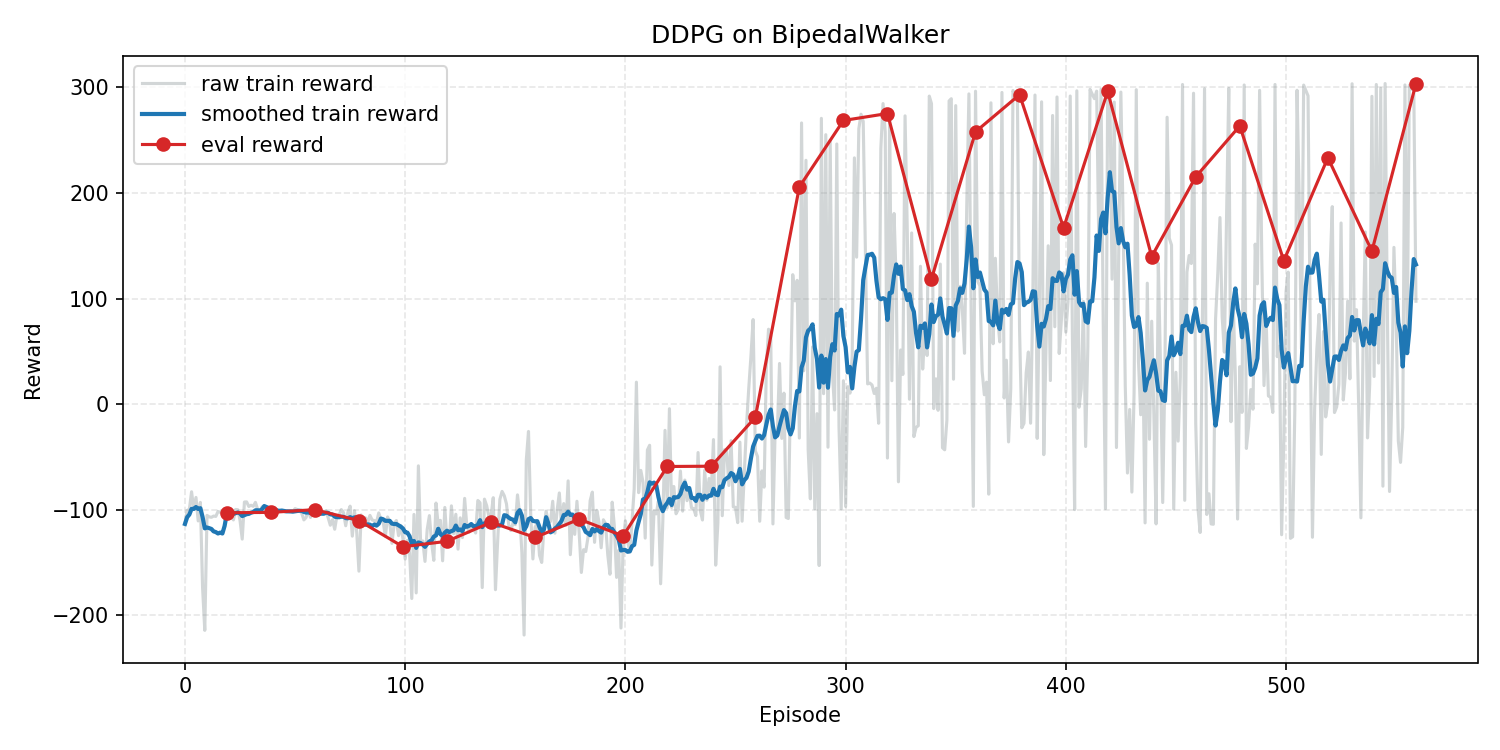
\includegraphics[width=0.92\linewidth]{training_curve.png}
\caption{DDPG在BipedalWalker上的训练曲线（灰色散点：原始回报；蓝色曲线：滑动平均回报，窗口$K=10$；红色圆点：无噪声评估回报，每20 episode评测一次）}
\label{fig:reward_curve}
\end{figure}

\subsection{分阶段分析}

根据训练曲线的演化特征，可将训练过程划分为6个典型阶段：

\begin{table}[H]
\centering
\caption{训练过程分阶段统计}
\label{tab:phase}
\begin{tabular}{cccccc}
\toprule
\textbf{阶段} & \textbf{Episodes} & \textbf{回报范围} & \textbf{平滑回报趋势} & \textbf{评估回报范围} & \textbf{阶段特征} \\
\midrule
初期探索 & 1--100 & [-214, -83] & $-138 \to -118$ & [-156, -103] & 频繁跌倒，随机探索为主 \\
挣扎期 & 101--200 & [-219, 21] & $-138 \to -139$ & [-136, -106] & 学习站立，回报波动大 \\
首次突破 & 201--280 & [-153, 275] & $-95 \to 12$ & [-59, 206] & 首次获得正回报，基本步态形成 \\
学习行走 & 281--380 & [-153, 297] & $13 \to 134$ & [118, 293] & 行走策略显著改善 \\
稳定行走 & 381--480 & [-113, 303] & $74 \to 82$ & [140, 293] & 步态趋于稳定 \\
收敛解决 & 481--560 & [-127, 303] & $35 \to 132$ & [136, 303] & 稳定达到求解标准 \\
\bottomrule
\end{tabular}
\end{table}

\subsection{关键里程碑事件}

\begin{table}[H]
\centering
\caption{训练过程中的关键里程碑}
\label{tab:milestones}
\begin{tabular}{cll}
\toprule
\textbf{Episode} & \textbf{事件} & \textbf{数值} \\
\midrule
206 & 首次获得正训练回报 & 20.79 \\
260 & 评估回报首次脱离负值 & $-12.48$ \\
280 & 评估回报突破200 & 205.77 \\
300 & 单episode训练回报突破270 & 275.28 \\
340 & 评估回报突破100 & 118.64 \\
360 & 评估回报突破250 & 257.98 \\
380 & 评估回报突破290 & 293.15 \\
420 & 评估回报接近300 & 296.19 \\
560 & \textbf{评估回报超过300，环境解决} & \textbf{303.49} \\
\bottomrule
\end{tabular}
\end{table}

\subsection{Loss变化分析}

训练过程中Actor Loss与Critic Loss的变化趋势如下：初期Critic Loss从14.95快速下降至3-5附近，表明Q值函数快速收敛；中期Actor Loss从-5逐渐降低至-26，表明策略持续优化；后期两者均趋于平稳，Loss值在小范围内波动，网络参数已达较优状态。

\section{结果分析}

\subsection{学习过程的时间演化规律}

依据图~\ref{fig:reward_curve}的回报曲线和表~\ref{tab:phase}的阶段统计，可以识别出双足机器人行走学习的三个关键转折点：

\paragraph{转折点一：首次正回报（Episode 206）}
在此之前，智能体累计回报始终低于-80，说明机器人频繁跌倒或无法有效前进。在经历了约200个episode（约90,000步）的探索后，智能体首次获得正回报20.79。这表明：
\begin{itemize}[leftmargin=2em]
  \item Actor网络经过约150个episode的有效更新后，开始输出足以维持身体平衡的关节扭矩组合；
  \item OU噪声的时间相关性在此起到了关键作用——它使得机器人在一个episode内可以维持相似的动作模式，而不是在每个时间步做完全随机的探索；
  \item 从物理角度理解，这一阶段对应机器人从"完全无法站立"到"能够短暂保持平衡并向前迈出一两步"的质变。
\end{itemize}

\paragraph{转折点二：评估回报突破200（Episode 280）}
从Episode 206到280仅经历了74个episode，但评估回报从-59跃升至205.77，提升了约450\%。这种非线性的快速提升反映了强化学习中的一个典型现象：\textbf{一旦策略越过了"能够站立"的阈值，学习速度会大幅加快}，因为此时回放池中的正样本比例急剧增加，Critic可以更准确地估计高回报状态的动作价值，Actor从而沿正确的梯度方向快速优化。

\paragraph{转折点三：评估回报稳定在290以上（Episode 380以后）}
从Episode 380开始，评估回报稳定在[140, 293]区间，单episode训练回报频繁达到290以上。这表明智能体已经掌握了在不同地形条件下自适应调整步态的能力。此时策略的主要波动来源于：\begin{inparaenum}
  \item 探索噪声引入的随机扰动；
  \item 环境地形随机生成导致的难度差异；
  \item Critic值函数在不同状态下的估计方差。
\end{inparaenum}

\subsection{算法组件的有效性分析}

\paragraph{Ornstein-Uhlenbeck噪声 vs. 高斯噪声}
在初次实验中，采用高斯噪声（$\sigma=0.15$）进行探索，训练400个episode后回报始终在-100附近徘徊，智能体未能学会任何有效策略。改用OU噪声（$\sigma=0.20, \theta=0.15$）后，智能体在560个episode内成功解决环境。这一对比表明：
\begin{itemize}[leftmargin=2em]
  \item OU噪声产生的时间相关探索序列更符合物理控制系统的惯性特性；
  \item 在BipedalWalker这类动作之间存在强连续依赖关系的任务中，相邻时间步保持相似的动作趋势比完全独立的随机扰动更有效；
  \item 从信号处理角度看，OU过程是低通滤波后的有色噪声，其频率成分更集中于低频，与双足行走的自然频率范围更匹配。
\end{itemize}

\paragraph{梯度裁剪与Critic学习率降低}
初次实验中Critic学习率设为$1\times10^{-3}$且未使用梯度裁剪，导致Actor Loss从$-6$持续增长至$-66$，表明Critic的Q值估计发生了发散。通过将Critic学习率降至$1\times10^{-4}$并添加梯度裁剪（$\max\_norm=1.0$），训练过程恢复稳定。这验证了文献~\cite{fujimoto2018td3}中的结论：\textbf{Critic学习率过大是DDPG训练不稳定的首要原因之一}。

\paragraph{细粒度更新策略}
将$\text{update\_iters}=50$改为$\text{update\_iters}=1$并配合$\text{update\_every}=1$，使得每次环境交互后仅进行一次网络更新。这种细粒度更新策略避免了单批数据上的过拟合风险，同时增加了参数更新的总频次，有利于更平稳地逼近最优策略。

\subsection{训练高方差现象分析}

从图~\ref{fig:reward_curve}可以观察到，相邻episode的训练回报波动幅度可达300以上（如Episode 278为97.81，Episode 280骤升至275.28，Episode 281又回调至-32.10）。这种高方差现象源于以下因素的叠加效应：
\begin{enumerate}[leftmargin=2em]
  \item \textbf{环境随机性}：\texttt{BipedalWalker-v3}的每个episode随机生成地形轮廓，平坦地形与崎岖地形之间的难度差异会导致回报产生本质区别；
  \item \textbf{探索噪声}：OU噪声的随机采样导致同一策略在不同episode中的表现差异；
  \item \textbf{初始状态扰动}：环境初始化时的小幅度随机扰动可能导致机器人初始姿态偏离，影响后续控制稳定性。
\end{enumerate}
这也是为什么评估回报（5个episode的平均值）比单episode训练回报更能反映策略真实水平的原因。

\section{工程问题剖析与解决对策}

\begin{table}[H]
\centering
\caption{训练过程中的工程问题与解决方案}
\label{tab:troubleshooting}
\begin{tabular}{p{2.8cm}p{3cm}p{3cm}p{3.2cm}}
\toprule
\textbf{故障现象} & \textbf{原因剖析} & \textbf{解决方案} & \textbf{经验总结} \\
\midrule
训练回报始终在$-100$附近，400ep未收敛 & 高斯噪声缺乏时间相关性；Critic学习率$10^{-3}$导致Q值发散；update\_iters=50导致过拟合 & 改为OU噪声（$\sigma=0.20$）；Critic学习率降至$10^{-4}$；update\_iters=1 & 连续控制任务优先选择OU噪声；Critic学习率通常应低于或等于Actor \\
\midrule
Actor Loss持续增长至$-66$ & Critic的Q值估计发散，梯度无约束 & 添加梯度裁剪（$\max\_norm=1.0$） & 梯度裁剪是DDPG训练的必备组件 \\
\midrule
训练回报出现极端低值（$-219$） & OU噪声在部分episode产生过大幅度的连续扰动 & 不处理（属于正常探索） & 偶发低回报是有效探索的代价，重点关注平滑后趋势 \\
\midrule
Buffer满后旧样本干扰 & 经验回放容量200k，旧策略样本过多 & 不处理（容量已较合适） & 缓冲区大小需与训练总步数匹配 \\
\bottomrule
\end{tabular}
\end{table}

\section{结论与展望}

\subsection{实验结论}

本实验基于DDPG算法在\texttt{BipedalWalker-v3}环境中实现了双足机器人行走策略的学习，得出以下主要结论：

\begin{enumerate}[leftmargin=2em]
  \item \textbf{DDPG能有效解决BipedalWalker连续控制任务}：经过560个episode的训练，评估平均回报达到303.49，超过300的求解阈值，测试平均回报303.28验证了策略的稳定性和泛化能力。
  \item \textbf{探索噪声策略对训练成败具有决定性影响}：时间相关的OU噪声（$\sigma=0.20$）显著优于独立同分布的高斯噪声，其物理合理性在于连续控制系统中相邻时间步的动作应具有连续性。
  \item \textbf{训练稳定性是DDPG工程落地的关键瓶颈}：通过降低Critic学习率、添加梯度裁剪、实施细粒度更新策略（update\_iters=1）以及引入目标策略平滑，有效解决了Q值发散和过拟合问题。
  \item \textbf{BipedalWalker的学习过程呈现清晰的阶段性特征}：从随机探索（0-200ep）→行走能力突破（200-280ep）→快速提升（280-380ep）→稳定收敛（380-560ep），每个阶段的转换对应着策略的质变。
\end{enumerate}

\subsection{未来工作展望}

本实验仍有以下改进方向可供探索：

\begin{itemize}[leftmargin=2em]
  \item \textbf{算法升级}：TD3\cite{fujimoto2018td3}通过双Critic和延迟策略更新进一步减少值函数高估偏差；SAC\cite{haarnoja2018sac}通过最大熵框架提升探索效率和鲁棒性。两者在BipedalWalker上通常能取得比DDPG更高的样本效率和更低的超参数敏感性。
  \item \textbf{噪声衰减策略}：当前采用固定方差OU噪声，训练后期仍保持强探索反而会干扰已收敛策略。引入随训练进程衰减的噪声方差有望加速收敛。
  \item \textbf{网络结构优化}：当前全连接网络结构较为基础。可考虑引入Layer Normalization、残差连接或LSTM时序建模，以提升网络表达能力和训练稳定性。
  \item \textbf{多随机种子统计}：当前训练仅在seed=42下进行一次。增加3-5个不同随机种子的重复实验，取均值和方差，可以更可靠地评估算法性能。
\end{itemize}

\begin{thebibliography}{99}

\bibitem{lillicrap2015ddpg}
Lillicrap T P, Hunt J J, Pritzel A, et al.
\newblock Continuous control with deep reinforcement learning.
\newblock \emph{arXiv preprint arXiv:1509.02971}, 2015.

\bibitem{silver2014dpg}
Silver D, Lever G, Heess N, Degris T, Wierstra D, Riedmiller M.
\newblock Deterministic policy gradient algorithms.
\newblock In: \emph{Proceedings of the 31st International Conference on Machine Learning}, 2014.

\bibitem{fujimoto2018td3}
Fujimoto S, Van Hoof H, Meger D.
\newblock Addressing function approximation error in actor-critic methods.
\newblock In: \emph{Proceedings of the 35th International Conference on Machine Learning}, 2018.

\bibitem{haarnoja2018sac}
Haarnoja T, Zhou A, Abbeel P, Levine S.
\newblock Soft actor-critic: Off-policy maximum entropy deep reinforcement learning with a stochastic actor.
\newblock In: \emph{Proceedings of the 35th International Conference on Machine Learning}, 2018.

\bibitem{mnih2015dqn}
Mnih V, Kavukcuoglu K, Silver D, et al.
\newblock Human-level control through deep reinforcement learning.
\newblock \emph{Nature}, 2015, 518(7540): 529--533.

\end{thebibliography}

\end{document}